%%%%%%%%%%%%%%%%%%%%%%%%%%%%%%%%%%%%%%%%%%%%%%%%%%%%%%%%%%%%%%%%
\begin{figure}
  \centering
  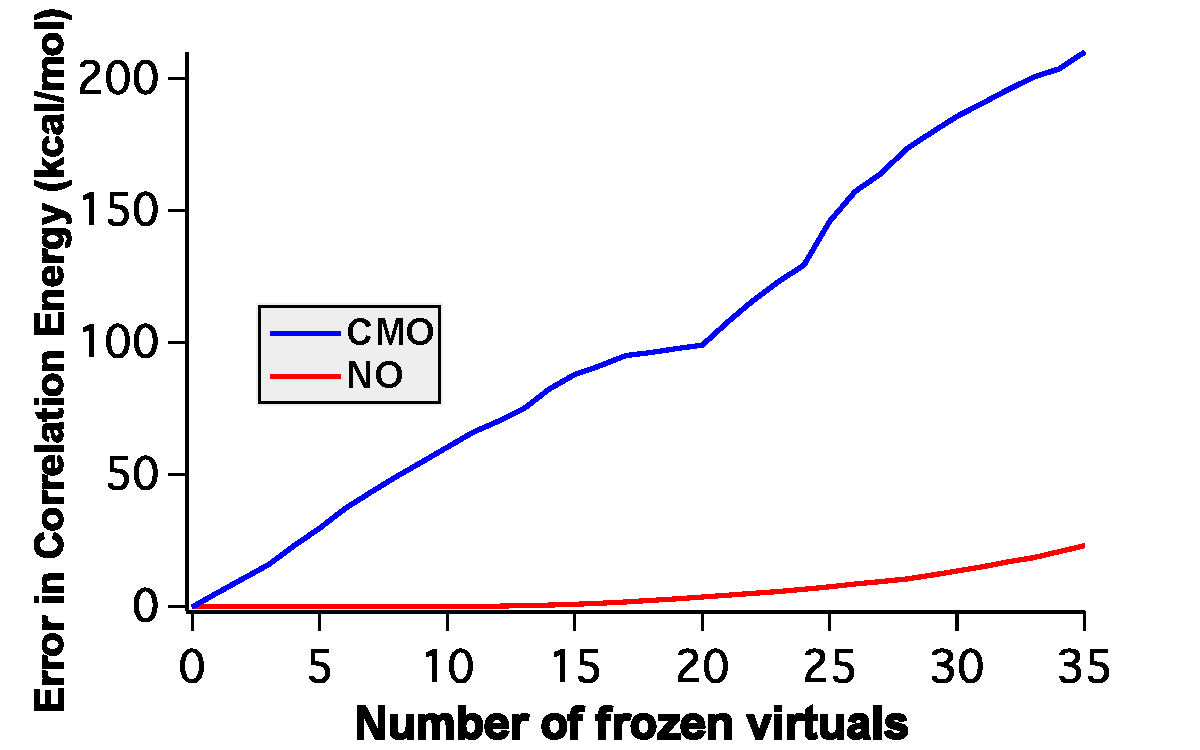
\includegraphics[width=0.7\linewidth]{figures/energy.pdf}
  \caption{Error in the CCSD energy of H$_2$O$_2$ in kcal/mol as a 
           function of the number of frozen virtual orbitals in both CMO and NO bases.} 
  \label{fig:energy}
\end{figure}
%%%%%%%%%%%%%%%%%%%%%%%%%%%%%%%%%%%%%%%%%%%%%%%%%%%%%%%%%%%%%%%
\begin{figure}
  \centering
  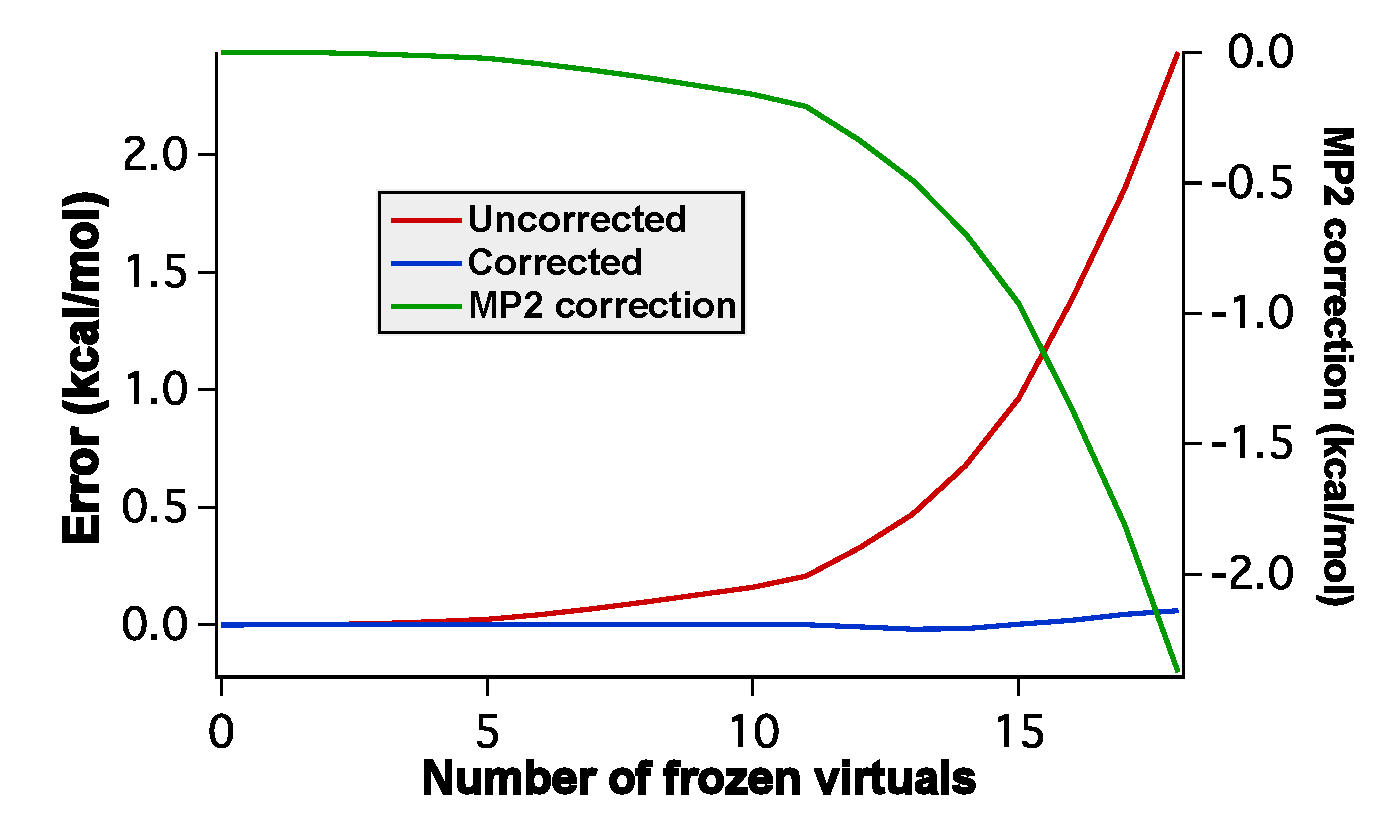
\includegraphics[width=0.7\linewidth]{figures/Mp2c.pdf}
  \caption{Error in CCSD energy of H$_2$O$_2$ in the NO bases, with and without MP2 corrections 
        and MP2 correction as a function of the number of frozen virtual orbitals.}
\label{fig:MP2_corr}
\end{figure}
%%%%%%%%%%%%%%%%%%%%%%%%%%%%%%%%%%%%%%%%%%%%%%%%%%%%%%%%%%%%%%%
\begin{figure}
  \centering
  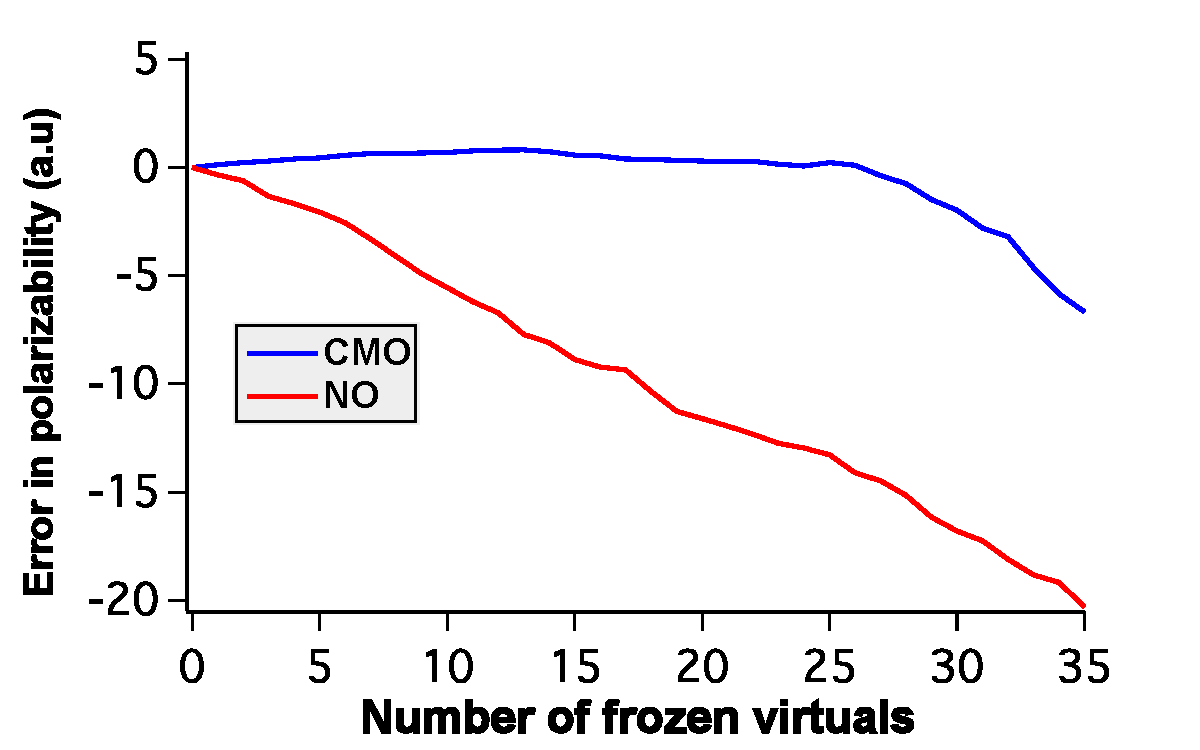
\includegraphics[width=0.6\linewidth]{figures/h2o2_polar.pdf}
  \caption{Errors in the CCSD/aDZ dynamic polarizability (589
nm) of H$_2$O$_2$ in 
       in both CMO and NO bases as a function of number of virtual orbitals removed.}
   \label{fig:polar_h2o2}
\end{figure}
%%%%%%%%%%%%%%%%%%%%%%%%%%%%%%%%%%%%%%%%%%%%%%%%%%%%%%%%%%%%%%%
\begin{figure}
  \centering
  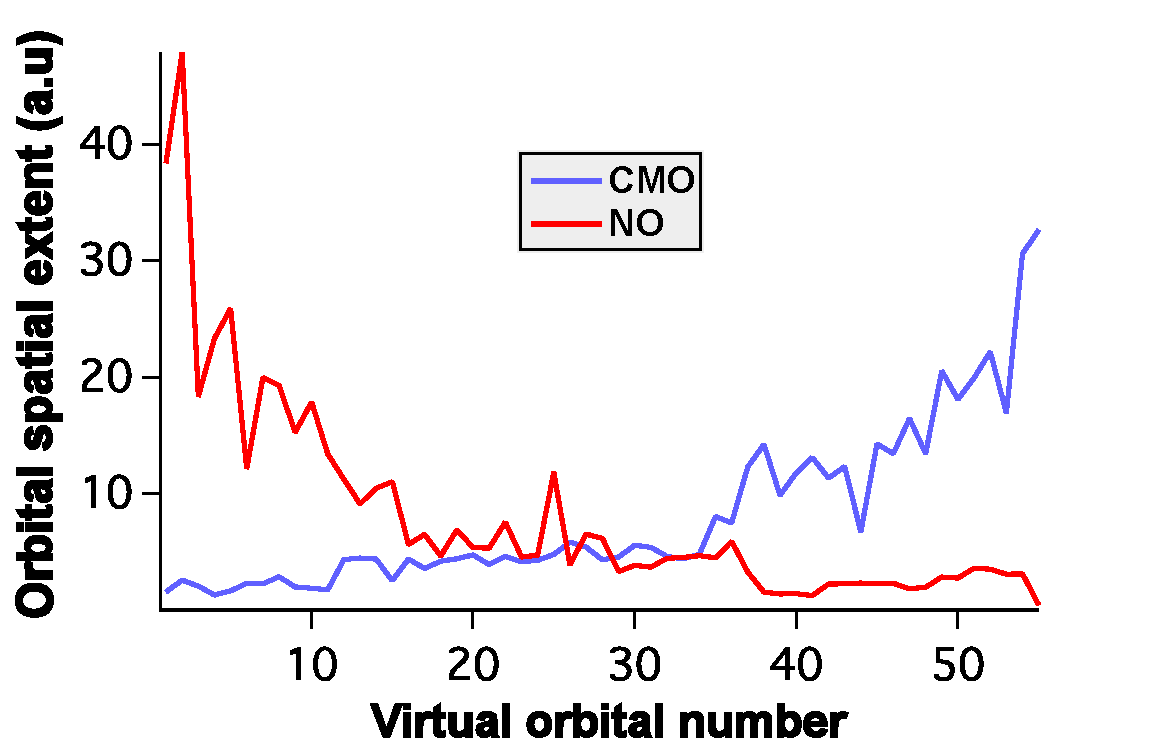
\includegraphics[width=0.6\linewidth]{figures/spatial.pdf}
  \caption{Spatial extent ($\langle r^2\rangle$) of virtual
orbitals of H$_2$O$_2$ in both CMO and NO bases.  Orbitals are ordered
left-to-right by
decreasing energy (CMOs) or increasing occupation number (NOs).}
   \label{fig:spatial}
\end{figure}

%%%%%%%%%%%%%%%%%%%%%%%%%%%%%%%%%%%%%%%%%%%%%%%%%%%%%%%%%%%%%%%
\begin{figure}
  \centering
  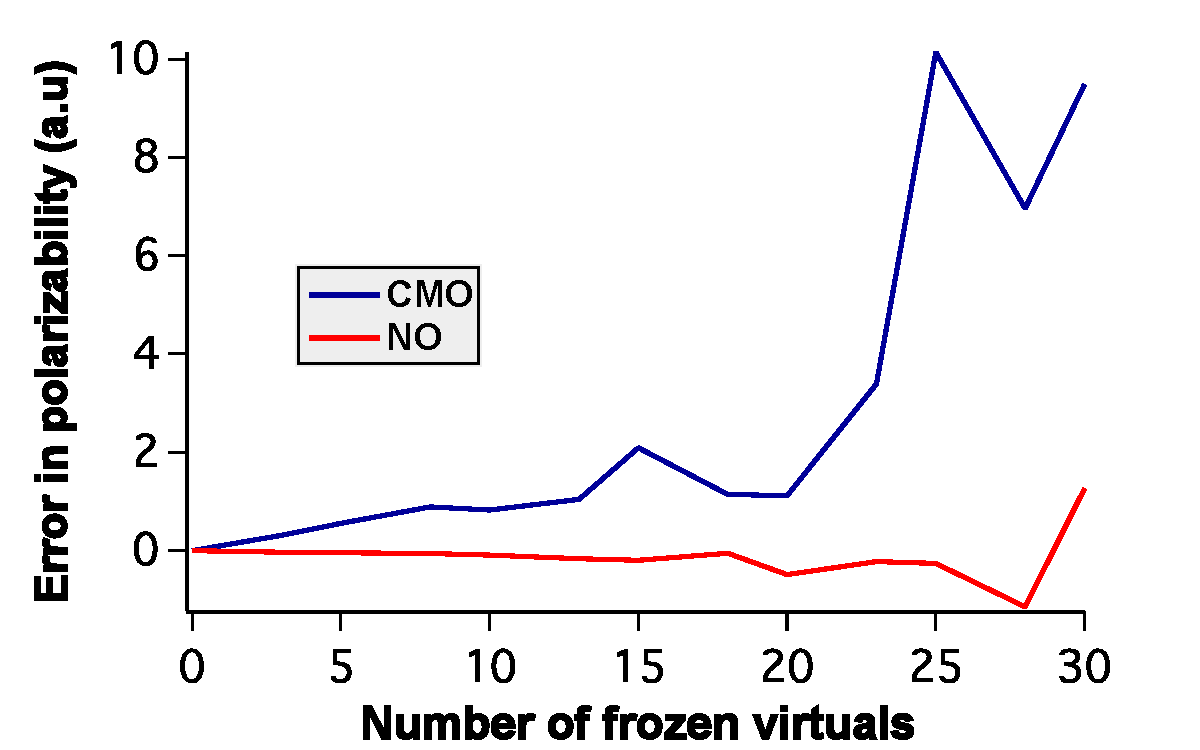
\includegraphics[width=0.6\linewidth]{figures/polar_static.pdf}
  \caption{Errors in the CCSD/aDZ static polarizability 
(including orbital relaxation effects) of H$_2$O$_2$ in
       in both CMO and NO bases as a function of number of virtual orbitals
removed.}
   \label{fig:static}
\end{figure}

%%%%%%%%%%%%%%%%%%%%%%%%%%%%%%%%%%%%%%%%%%%%%%%%%%%%%%%%%%%%%%%
\begin{figure}
  \centering
  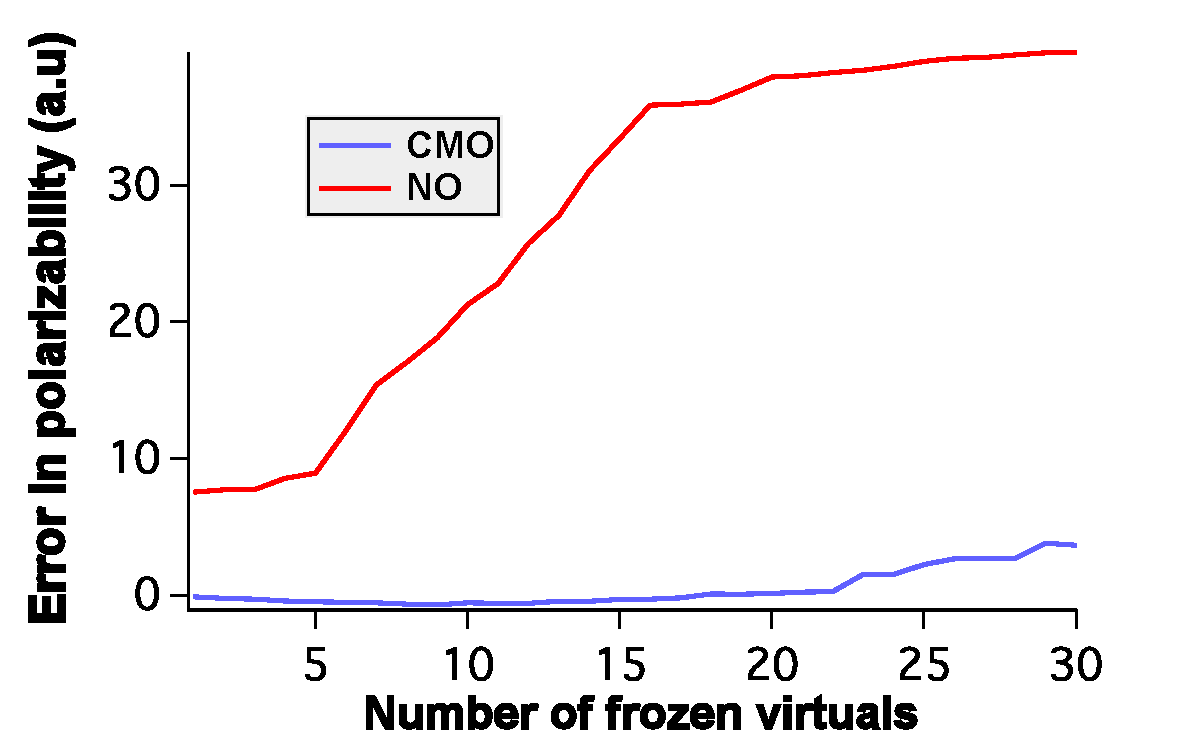
\includegraphics[width=0.6\linewidth]{figures/sort_spatial.pdf}
  \caption{Errors in the CCSD/aDZ dynamic polarizability (589
nm) of H$_2$O$_2$ as a function of the number of virtual CMOs or NOs deleted,
ordered by increasing spatial extent, $\langle r^2 \rangle$.}
   \label{fig:sort_spatial}
\end{figure}
%%%%%%%%%%%%%%%%%%%%%%%%%%%%%%%%%%%%%%%%%%%%%%%%%%%%%%%%%%%%%%%
\begin{figure}
  \centering
  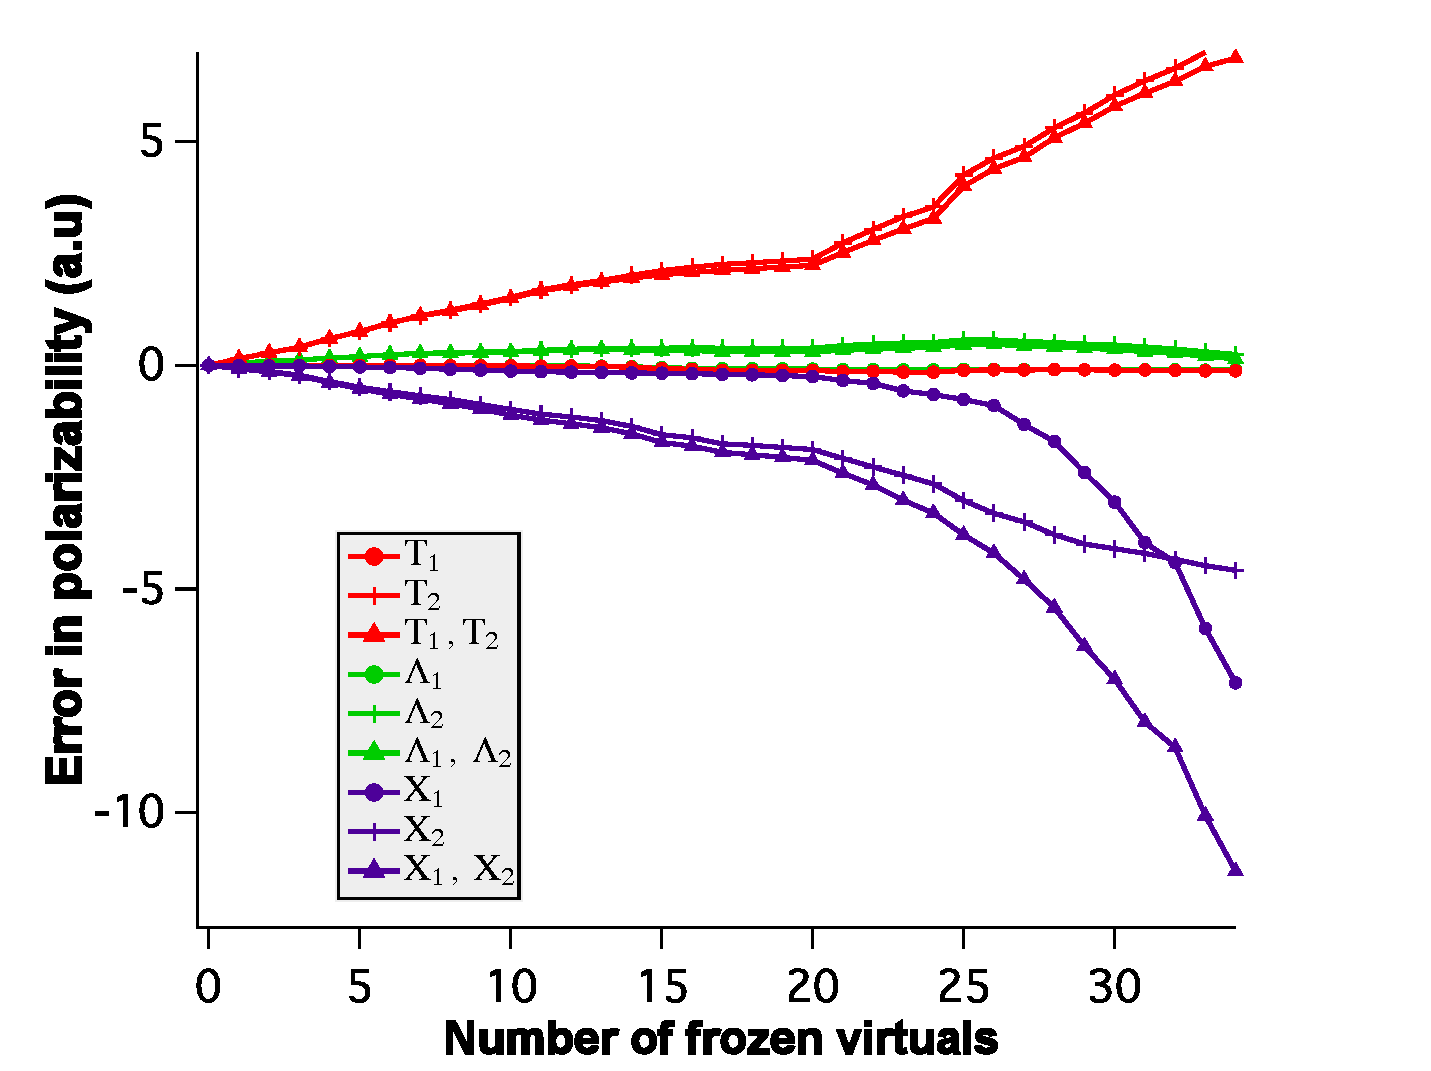
\includegraphics[width=0.6\linewidth]{figures/amp_trunc_cmo.pdf}
  \caption{Errors introduced in CCSD/aDZ polarizabilities of
H$_2$O$_2$ in the virtual CMO bases by the truncation of different classes of wave
function amplitudes.}
   \label{fig:amp_trunc_cmo}
\end{figure}
%%%%%%%%%%%%%%%%%%%%%%%%%%%%%%%%%%%%%%%%%%%%%%%%%%%%%%%%%%%%%%%
\begin{figure}
  \centering
  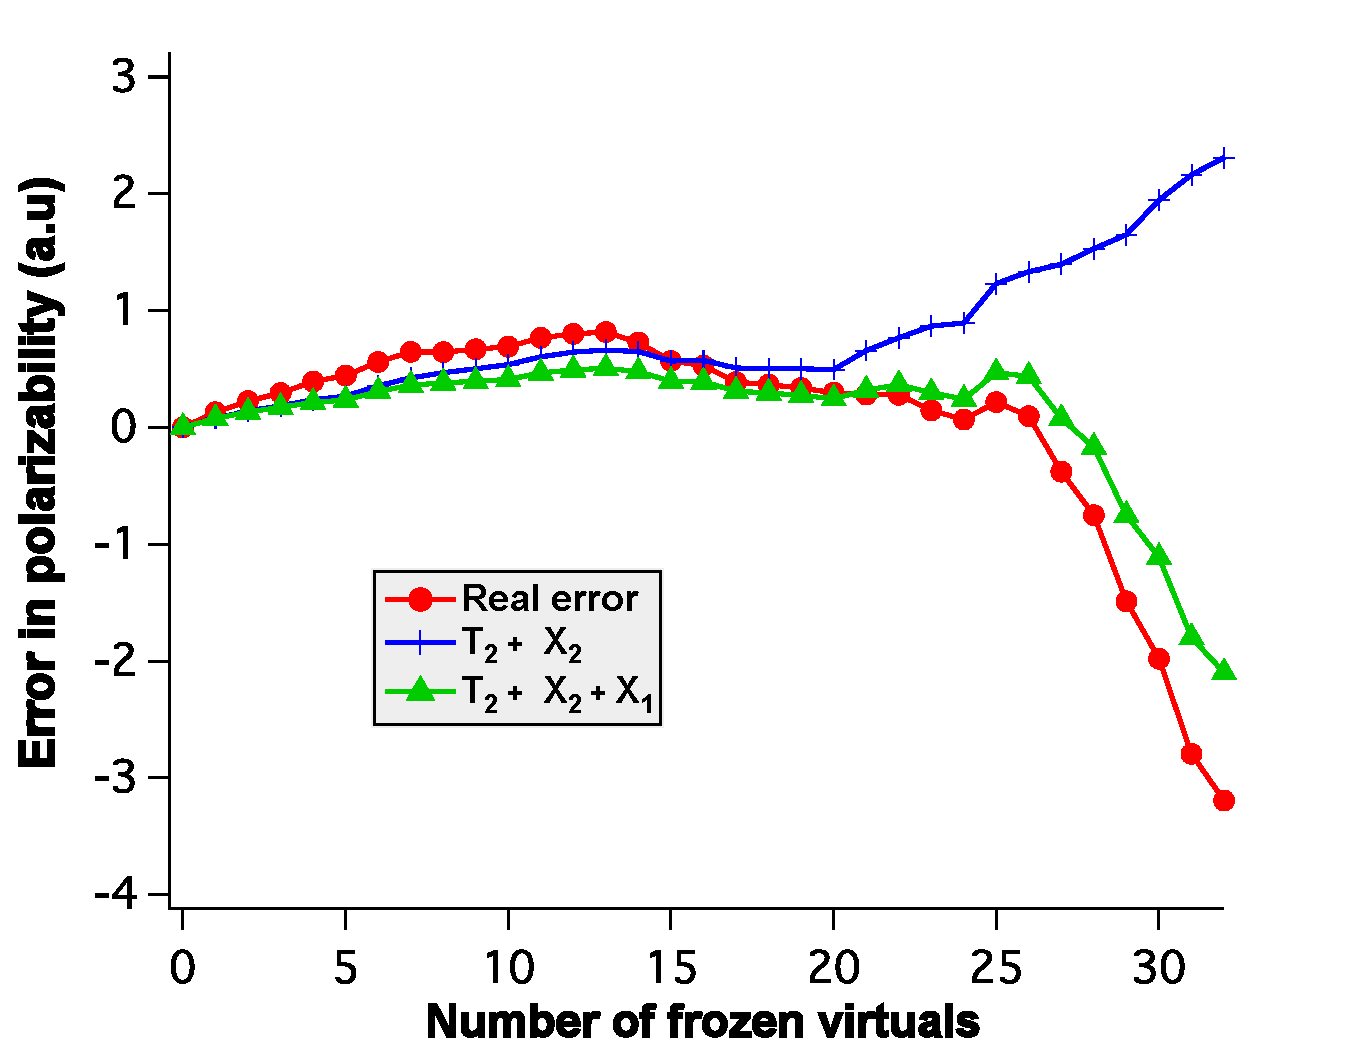
\includegraphics[width=0.6\linewidth]{figures/error_cmpare.pdf}
  \caption{Errors introduced in CCSD/aDZ polarizabilities of
H$_2$O$_2$ in the virtual CMO bases by the truncation of specific classes of wave
function amplitudes as compared to the total errors obtained by freezing of
virtual CMOs.}
   \label{fig:error_compare}
\end{figure}
%%%%%%%%%%%%%%%%%%%%%%%%%%%%%%%%%%%%%%%%%%%%%%%%%%%%%%%%%%%%%%%
\begin{figure}
  \centering
  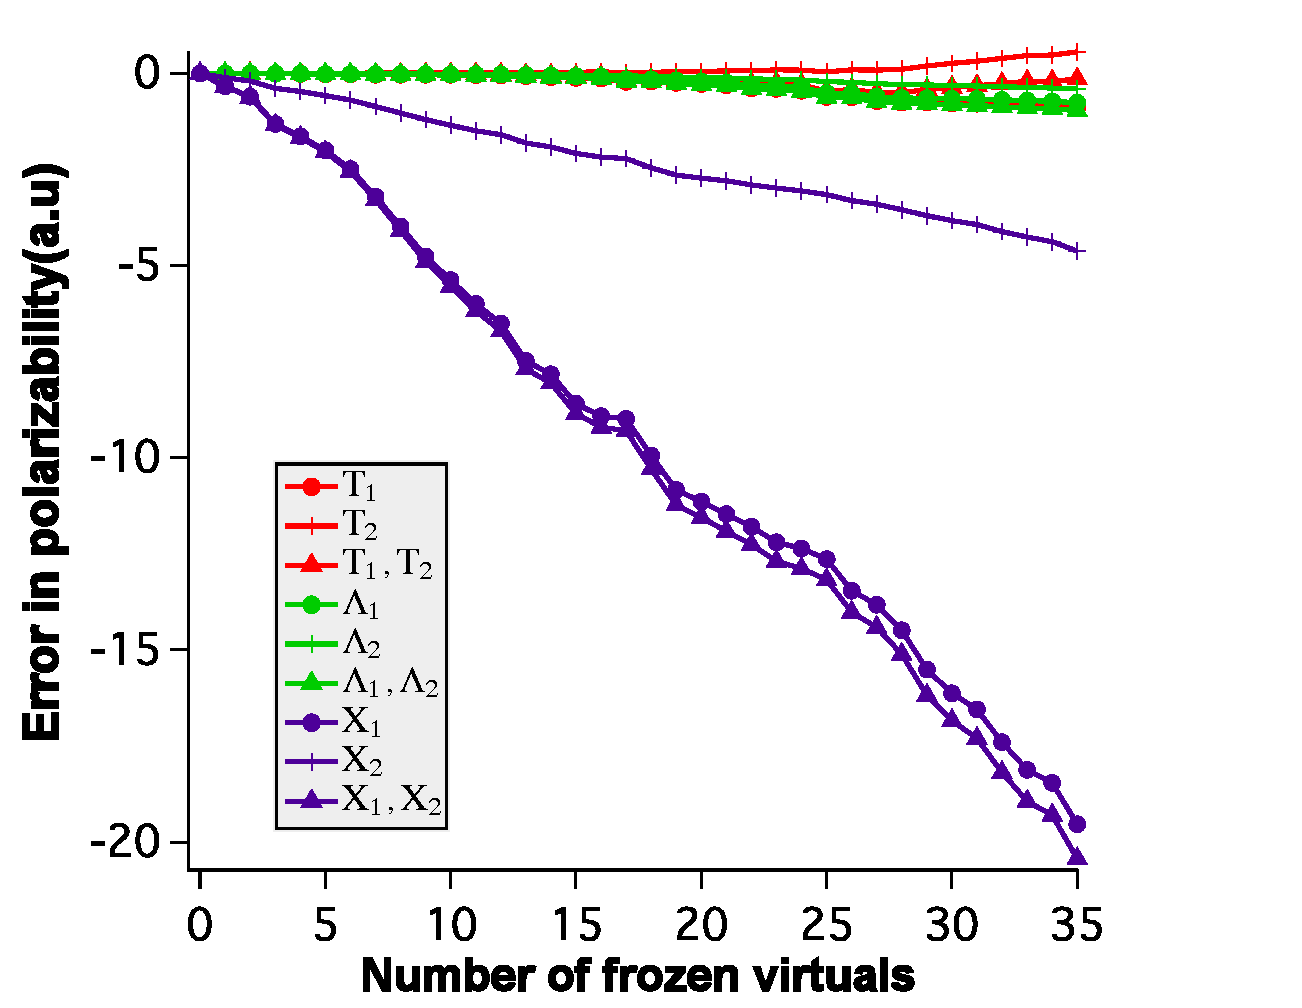
\includegraphics[width=0.6\linewidth]{figures/amp_trunc_no.pdf}
  \caption{Errors introduced in CCSD/aDZ polarizabilities of
H$_2$O$_2$ in the virtual NO bases by the truncation of different classes of wave
function amplitudes.}
   \label{fig:amp_trunc_no}
\end{figure}
%%%%%%%%%%%%%%%%%%%%%%%%%%%%%%%%%%%%%%%%%%%%%%%%%%%%%%%%%%%%%%%
\begin{figure}
  \centering
  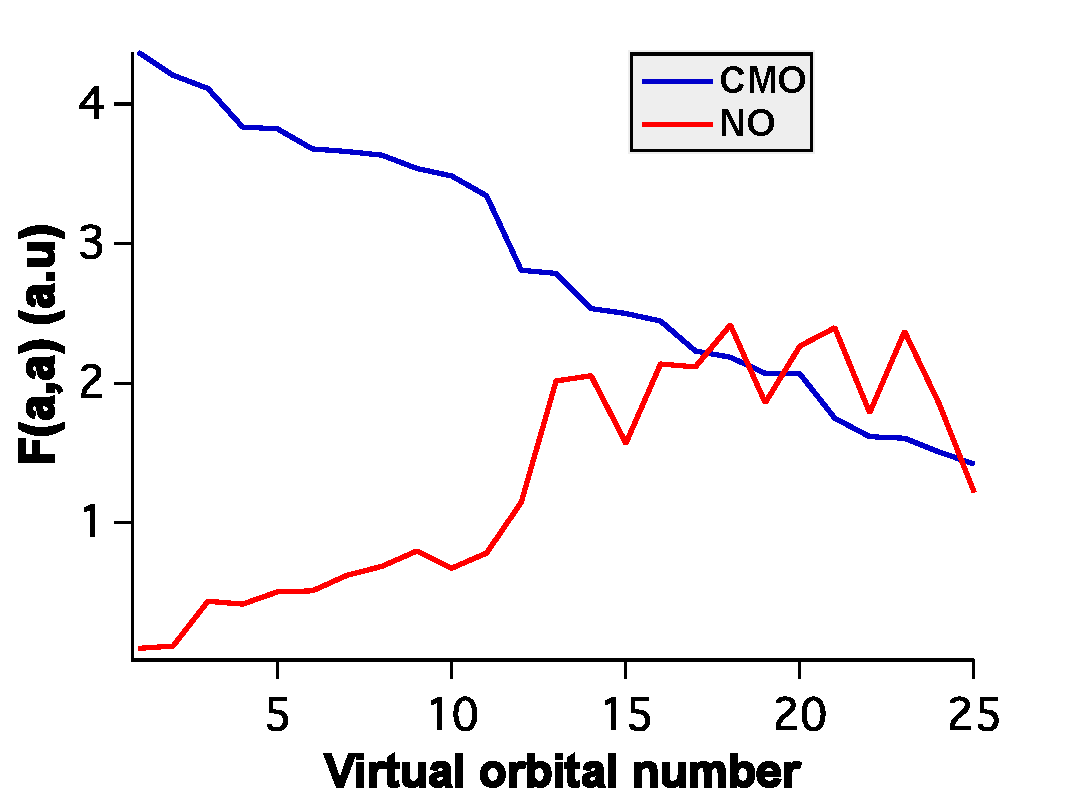
\includegraphics[width=0.6\linewidth]{figures/Faa.pdf}
  \caption{Virtual diagonal elements (a.u.) of the Fock matrix in
the CMO and NO bases.}
   \label{fig:Faa}
\end{figure}
%%%%%%%%%%%%%%%%%%%%%%%%%%%%%%%%%%%%%%%%%%%%%%%%%%%%%%%%%%%%%%%
\begin{figure}
  \centering
  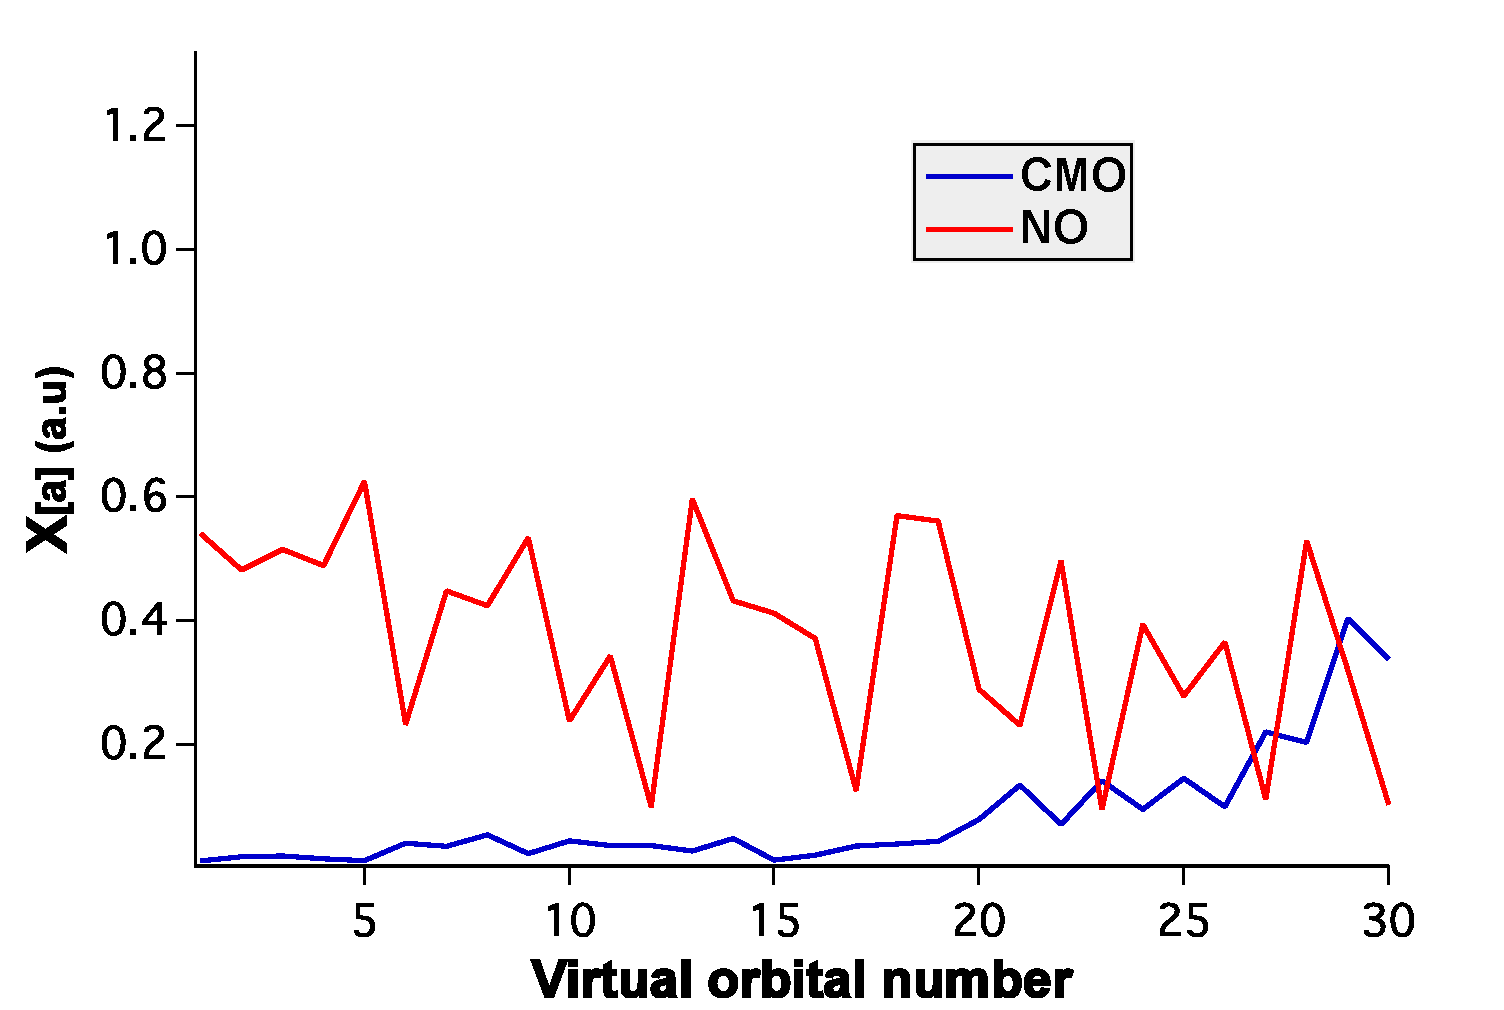
\includegraphics[width=0.6\linewidth]{figures/X1.pdf}
  \caption{Sum of the absolute values of $\hat{X}_1$
amplitudes for a given virtual, $\sum_i \left|X_i^a\right|$, for perturbation $\mu_x$
and frequency 589 nm, plotted for each virtual NO or CMO.}
   \label{fig:X1}
\end{figure}
%%%%%%%%%%%%%%%%%%%%%%%%%%%%%%%%%%%%%%%%%%%%%%%%%%%%%%%%%%%%%%%
\begin{figure}
  \centering
  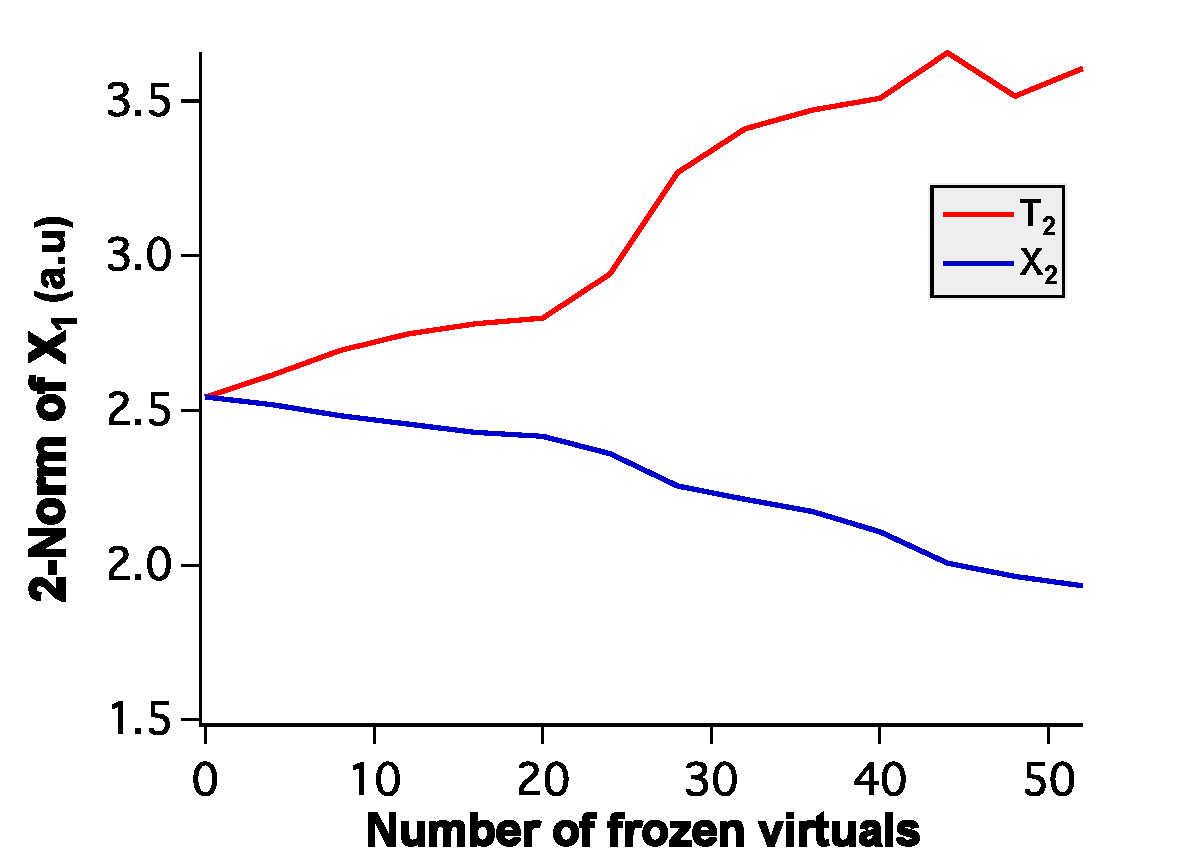
\includegraphics[width=0.6\linewidth]{figures/norm.pdf}
  \caption{The 2-norm of the $\hat{X}_1$ amplitude vector in
the CMO bases as a function of the truncation of classes of unperturbed 
$\hat{T}_2$ and perturbed $\hat{X}_2$ amplitudes.}
   \label{fig:norm}
\end{figure}
%%%%%%%%%%%%%%%%%%%%%%%%%%%%%%%%%%%%%%%%%%%%%%%%%%%%%%%%%%%%%%%
%\begin{figure}
%  \centering
%  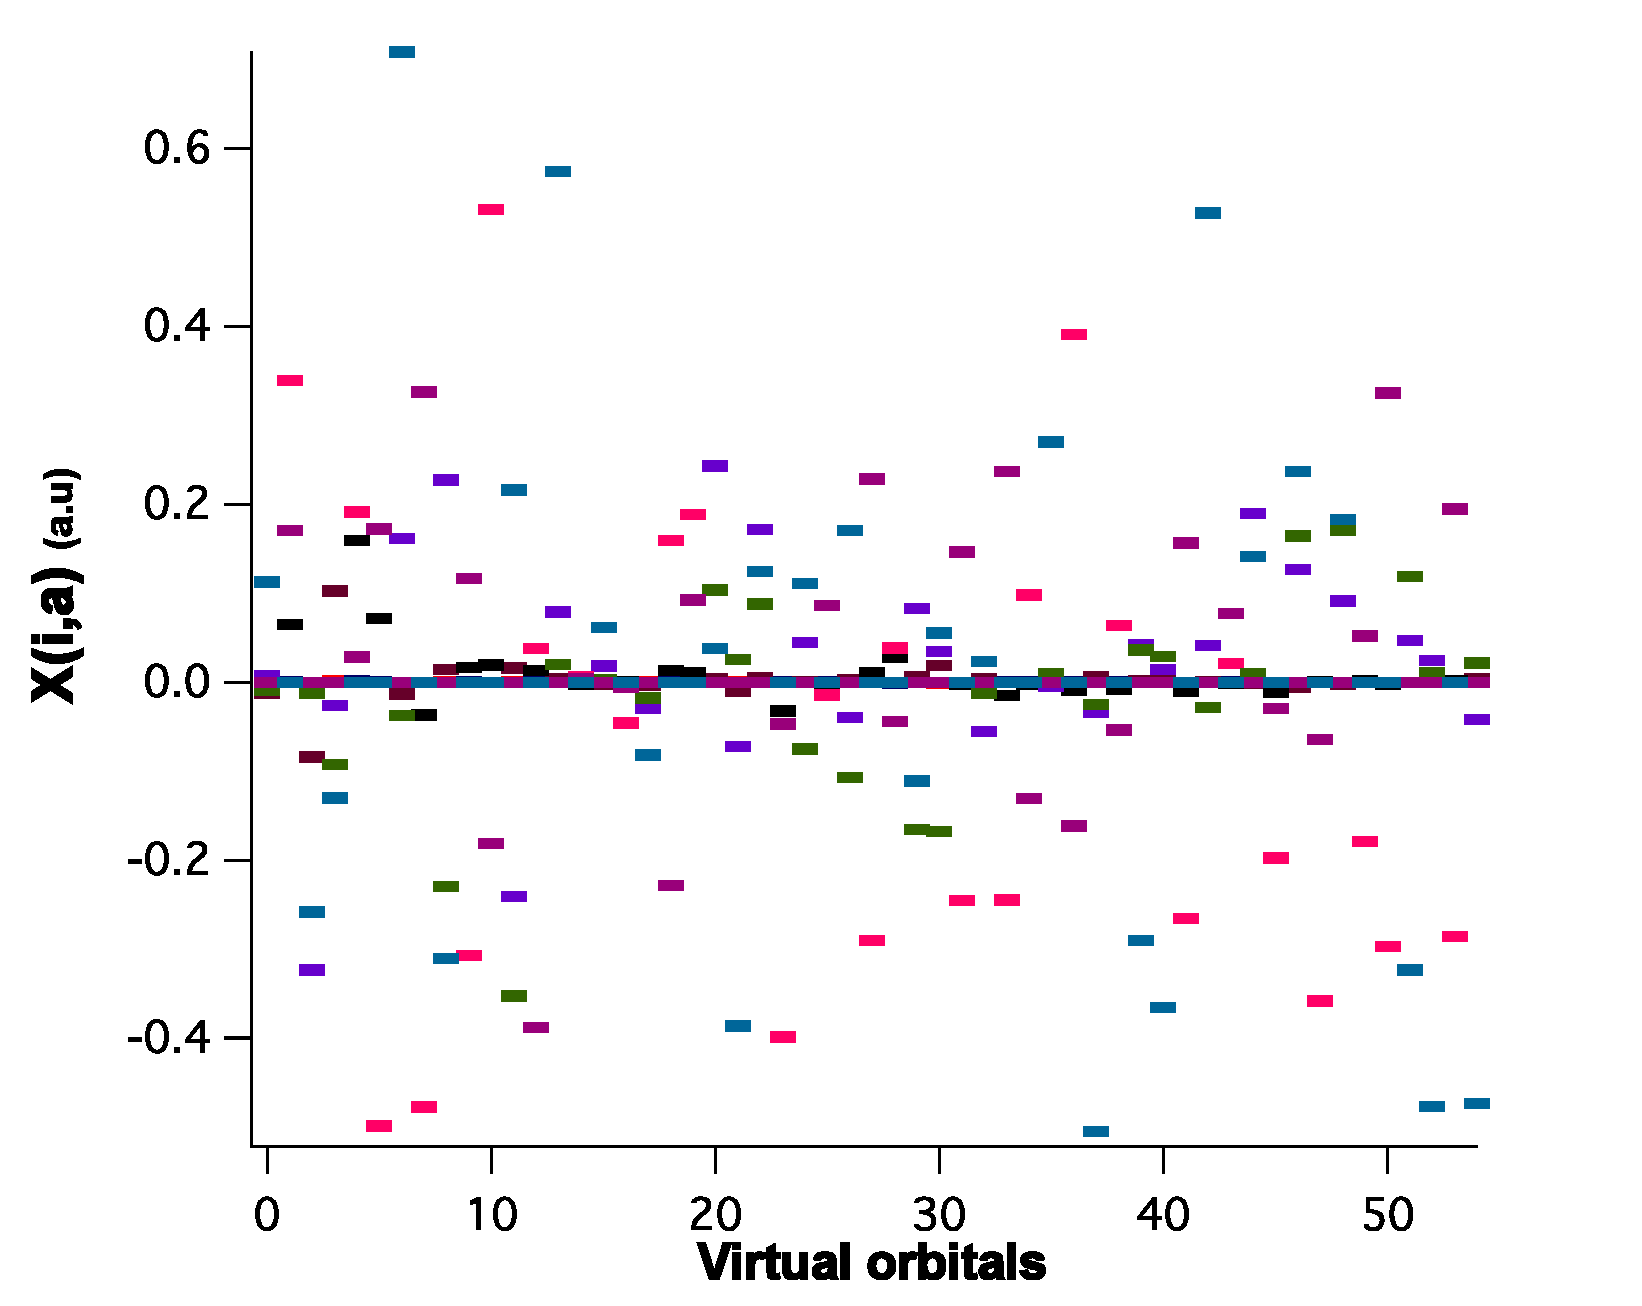
\includegraphics[width=0.6\linewidth]{figures/X1_no.pdf}
%  \caption{\footnotesize{$X_1$ amplitudes $X^{\mu_x}_{ia}$(589 nm) in the NO basis. For each virtual orbital there are nine virtual-occupied pairs.}}
%   \label{fig:X1_no}
%\end{figure}
%%%%%%%%%%%%%%%%%%%%%%%%%%%%%%%%%%%%%%%%%%%%%%%%%%%%%%%%%%%%%%%
\begin{figure}
  \centering
  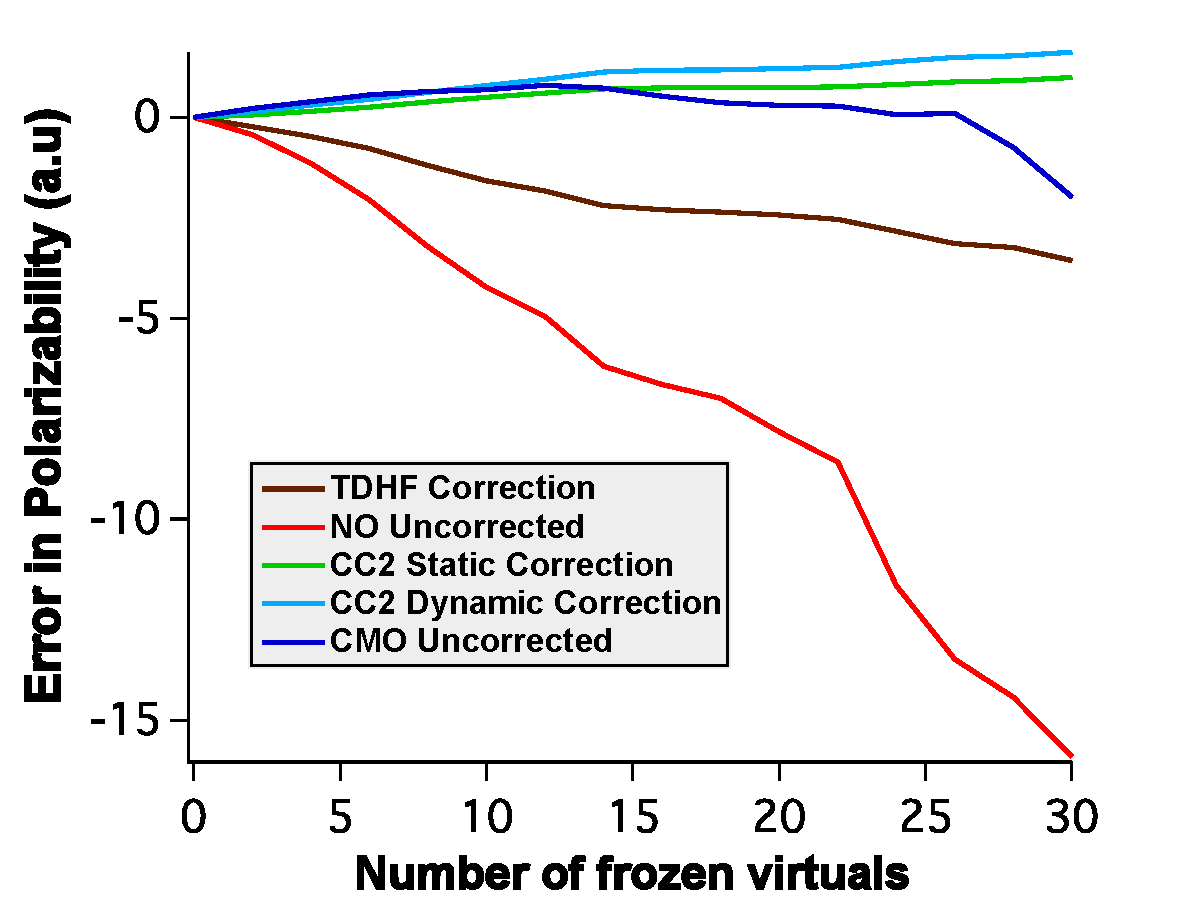
\includegraphics[width=0.6\linewidth]{figures/correctn.pdf}
  \caption{Correction schemes for the external truncated
NO space for the CCSD/aDZ polarizabilities of H$_2$O$_2$.}
   \label{fig:corrections}
\end{figure}
%%%%%%%%%%%%%%%%%%%%%%%%%%%%%%%%%%%%%%%%%%%%%%%%%%%%%%%%%%%%%%%

\begin{figure}
  \centering
  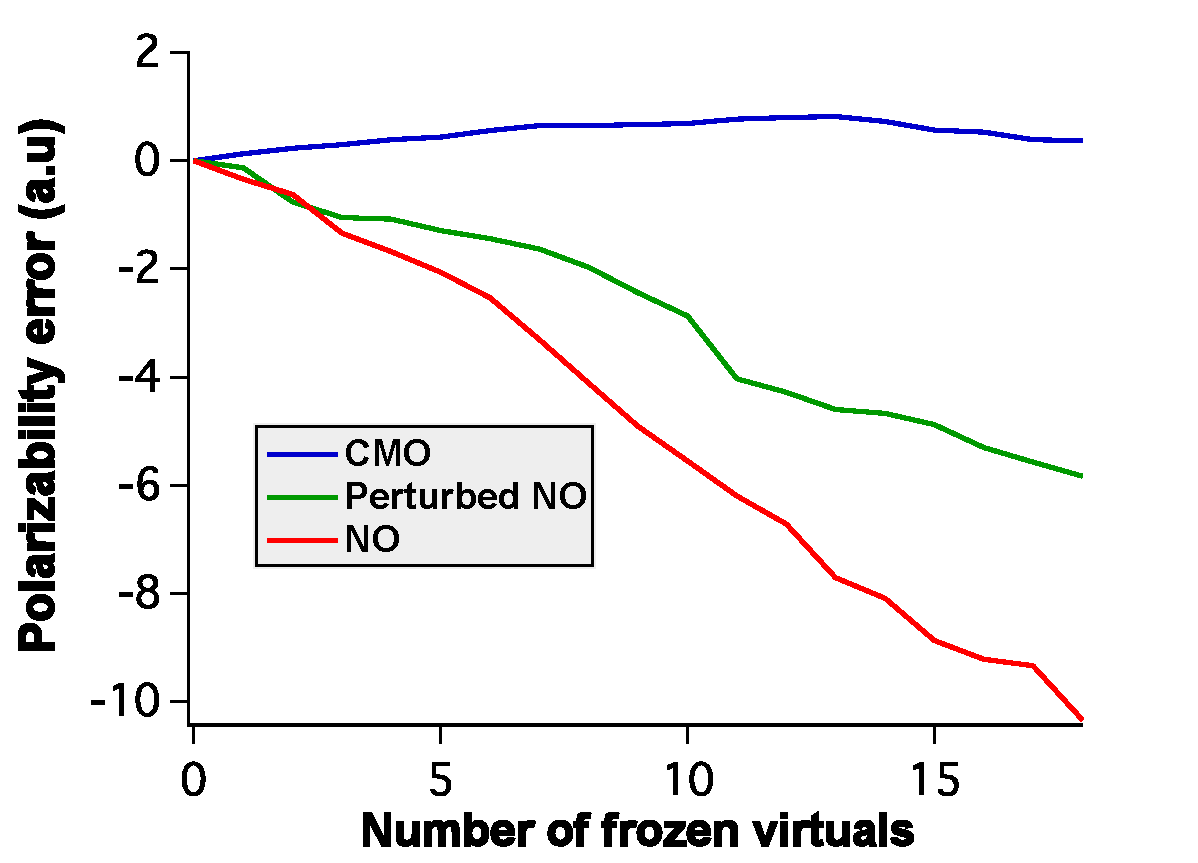
\includegraphics[width=0.6\linewidth]{figures/perturbed.pdf}
  \caption{Errors introduced in CCSD/aDZ polarizabilities of
H$_2$O$_2$ in the virtual CMO and NO bases, as well as the perturbed
virtual NO basis as a function of number of virtual orbitals removed.}
   \label{fig:perturb}
\end{figure}
%%%%%%%%%%%%%%%%%%%%%%%%%%%%%%%%%%%%%%%%%%%%%%%%%%%%%%%%%%%%%%%
\begin{figure}
  \centering
  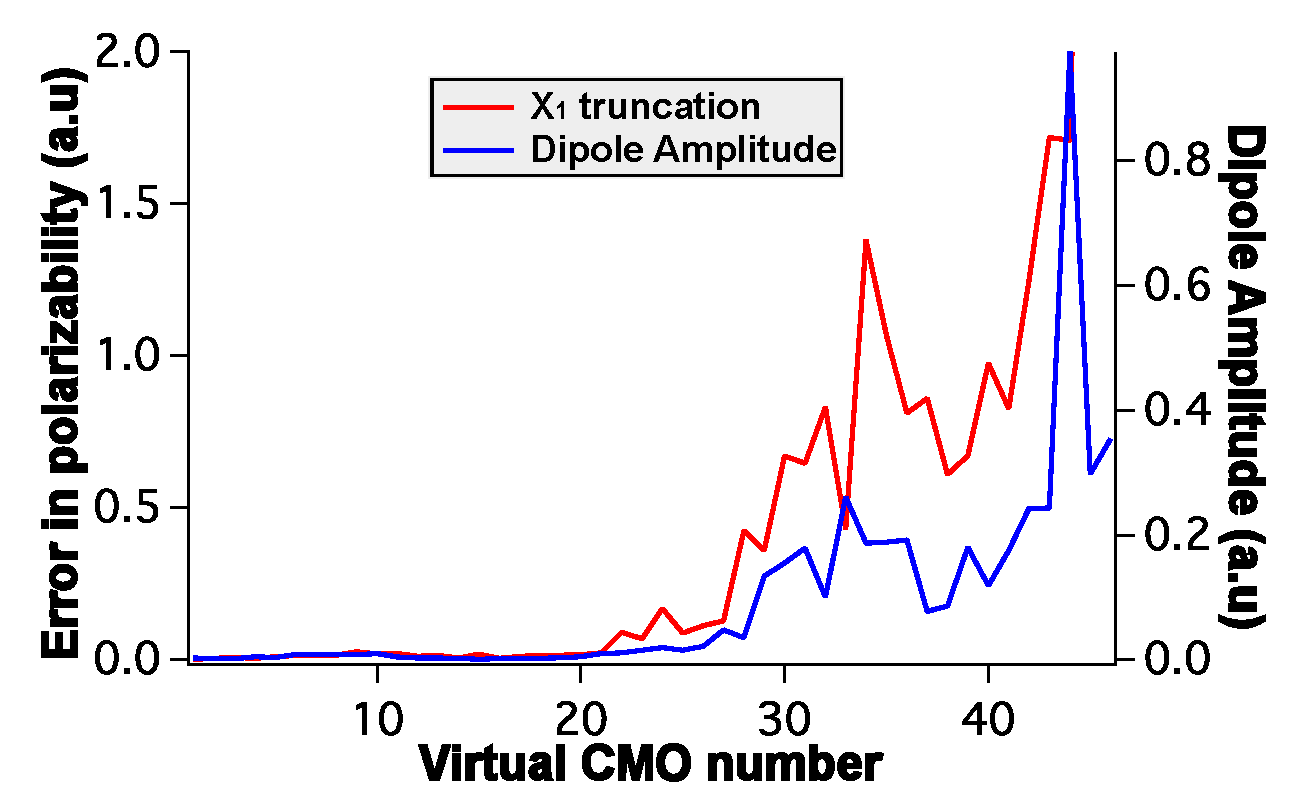
\includegraphics[width=0.6\linewidth]{figures/diplength.pdf}
  \caption{Absolute errors introduced in CCSD/aDZ
  polarizabilities of H$_2$O$_2$ due to truncation of $\hat{X}_1$ amplitudes and
  dipole amplitudes plotted as a function of different virtual CMOs.}
   \label{fig:dipole_length}
\end{figure}
%%%%%%%%%%%%%%%%%%%%%%%%%%%%%%%%%%%%%%%%%%%%%%%%%%%%%%%%%%%%%%%


\newpage
\begin{center}
{\bf TOC Graphic}
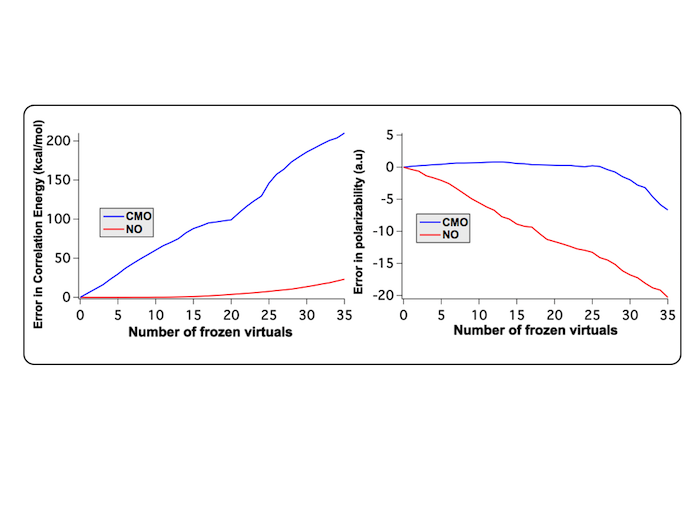
\includegraphics[width=1.0\linewidth]{figures/toc.png}
\end{center}
